\chapter{Higher-order correlation functions between kSZ and 21cm observations}
\label{chapter:ksz_21cm}

In Chapter~\ref{chapter:eor_intro}, it was discussed that there are many probes of the EoR beyond {\sc hi}. Secondary anisotropies of the CMB can be used as probes of reionization, mainly due to the fact that reionization represents a large source of free electrons, which CMB photons can scatter off of. The pattern of scattering -- the secondary anisotropies -- is sensitive to the topology of the {\sc hi} field. This Chapter focuses on a particular mechanism for producing secondary anisotropies; the kinetic Sunyaev-Zel'dovich effect (kSZ). We present novel mathematical theories or understanding the correlation between future CMB and EoR measurements, taking instrumental noise and the EoR window into account in a way not presently explored in the literature. In Section~\ref{sec:ksz-21cm} we make clear the link between the EoR and the kSZ effect, and the separate challenges to detecting either. In Sections~\ref{sec:bispec} and \ref{sec:trispec}, we present semi-analytic theory and results from simulation for the kSZ$^2$-21cm bispectrum and the kSZ$^2$-21cm$^2$ trispectrum, respectively.

\section{The kSZ-21cm connection}
\label{sec:ksz-21cm}

The kSZ probes the cosmic momentum field; photons are Doppler-boosted off of clouds of electrons around ionizing sources. The 21\,cm signal, of course, probes where those ionizing sources \textit{are not}, so we should expect the kSZ and 21\,cm signal to be anti-correlated. 

The anisotropies induced on the CMB by the kSZ is given by (Equation~\ref{eq:eor_intro_ksz}):
\begin{equation}
\frac{\delta T_{\rm kSZ}}{T_{\rm CMB}}(\hat{s}) = \frac{\sigma_T}{c} \int_0^{z_{\rm recomb}} n_e(z)e^{-\tau(z)} \hat{s}\cdot\vec{q} \frac{{\rm d}s}{{\rm d}z}{\rm d}z,
\end{equation}
where $\sigma_T$ is the Thomson Cross Section, $n_e(z)$ is the average number density of electrons at redshift $z$, $\tau(z)$ is the optical depth to redshift $z$, and d$s$/d$z$ is the cosmological line element to redshift $z$ along direction $\hat{s}$. 
The momentum field $q$ can be expressed as:
\begin{equation}
\vec{q}(\hat{s}) = (1+\delta_x)(1+\delta_b)\vec{v}(\hat{s}),
\end{equation}
where  $1+\delta_x = x_i/\left\langle x_i \right\rangle$, $1+\delta_b= \rho_b/\left\langle \rho_b \right\rangle$, $\vec{v}$ is the free electron bulk flow, and $\left\langle ... \right\rangle$ indicates an average over position $\vec{x}$. 
The kSZ is sourced by momentum of ionized gas, but we only detect the component of that momentum over a given line-of-sight $\hat{n}$, of which only the integrated, transverse component of the wavevector $\vec{k}$ will survive.
This representation allows us to approximate $\delta T_{\rm kSZ}$ as
\begin{align}
\delta T_{\rm kSZ} &\propto \vec{q}\cdot\hat{n}(\vec{k}) = \vec{v}(\vec{x})\left[1 + \delta_x(\vec{x}) + \delta_{\rho}(\vec{x})\right]\cdot\hat{n}(\vec{k})\\
\times & \int \frac{{\rm d}^3k'}{(2\pi)^3}\vec{v}(\vec{k}')\hat{k}'\cdot\hat{n}\left[\delta_x(\vec{k}-\vec{k}') + \delta_{\rho}(\vec{k}-\vec{k}')\right].
\end{align}
where the constant of proportionality can be expressed as a window function, described below in Equation~\ref{eq:WkSZ}. 

Likewise, the 21\,cm brightness temperature as a function of position can be expressed as (see Chapter~\ref{chapter:eor_intro}):
\begin{equation}
\delta_{\rm 21cm}(\vec{x}) \approx T_0^{\rm 21cm} \left\langle x_{\sc hi} \right\rangle \left[1 + \delta_{x_{\rm HI}}(\vec{x})\right] \left[1 + \delta_\rho(\vec{x})\right]
\label{eq:d21cm}
\end{equation}
To compare with the kSZ, it will be useful to speak in terms of the ionization overdensity field rather than neutral overdensity $\delta_{x_{\sc hi}}(\vec{x})$. This just brings out a prefactor,
\begin{equation}
\delta_{x_{\sc hi}}(\vec{x}) = \frac{-\langle x_i \rangle}{1 - \langle x_i \rangle} \delta_x(\vec{x}).
\end{equation}
So our representation of the 21\,cm temperature contrast becomes
\begin{equation}
\delta_{\rm 21cm}(\vec{x}) = T_0^{\rm21cm} (1 - \langle x_i \rangle ) \left[ 1 - \frac{\langle x_i \rangle}{1 - \langle x_i \rangle} \delta_x(\vec{x}) + \delta_{\rho}(\vec{x})  - \frac{\langle x_i \rangle}{1 - \langle x_i \rangle} \delta_x(\vec{x}) \delta_{\rho}(\vec{x}) \right]
\label{eq:d21cm_x}
\end{equation}

In the proceeding sections, we form higher-order correlation functions represented as bispectra (the Fourier analog of the three-point function) and trispectra (the four-point function). The reason for moving higher than the power spectrum (the two-point function) was because while the 21\,cm field is positive-definite, the kSZ anisotropies are not. Cosmic bulk flows could be oriented towards or away from the observer, and averaging the kSZ over the field would heavily attenuate it. Therefore, we required at least the square of the kSZ field -- and thus a move to higher-order statistics.

To simplify the mathematical derivations, we made a few simplifying assumptions: (i) at high redshifts, peculiar velocities along the line-of-sight were small compared to the Hubble Flow, (ii) X-ray heating effects close to the start of reionization pushed the spin temperature of {\sc hi} $T_S \gg T_{\rm CMB}$ \citep[e.g.][]{Meiksin.17}, and (iii) the velocity field was coherent on large scales \citep[e.g.][]{Smith.16}.

\subsection{Foregrounds}

As discussed throughout this work, the major foreground EoR experiments face is bright Galactic and extragalactic synchrotron. We ignore polarization contamination for this Chapter. In Section~\ref{sec:bispec}, we will show that the bispectrum, while theoretically and computationally tangible, is extremely sub-optimal in the context of 21\,cm observations, forcing the power measured to be sourced from within the wedge. The study of the trispectrum, presented in Section~\ref{sec:trispec}, was motivated by this limitation and overcomes it in a rather elegant fashion.

Foreground challenges for the kSZ exist on large scales as the primary CMB anisotropies and the secondary ones from the thermal Sunyaev-Zeldovich effect, and on small scales as the far-infrared background (FIB). Both of these foregrounds are minimal around multipoles $\ell 3000 - 6000$. The FIB effectively manifests as a shot-noise term in CMB maps, and could reasonably be windowed or subtracted to allow access to multipoles out to $\ell\sim 13,000$ for near-future CMB surveys (known as `Stage 3 and 4' in the cosmology community; \citealt{cmbS4.16}).

\subsection{Noise Estimates}

The single bispectrum triangle or trispectrum rectangle (see Sections~\ref{sec:bispec} and \ref{sec:trispec} respectively) will depend on the $C_{\ell}$ spectrum of noise arising from CMB and 21\,cm experiments. 

For the CMB, as noted above, measurements at appropriate $\ell$ values will leave the FIB as the dominant noise source. The minimum value of this term was reported by \cite{George.15} as 
\begin{equation}
\hat{D}_{\ell = 3501 - 3900} = \left\langle \frac{\ell(\ell+1)}{2\pi}C_{\ell} \right\rangle_{\ell = 3501 - 3900} = 30.8\pm 1.2\mu {\rm K}^2.
\end{equation}

\subsubsection{$C_{\ell}$ noise for HERA}

Massively-redundant interferometers typically make for poor imaging instruments, since they probe a relatively small number of $uv$ modes (e.g. Chapter~\ref{chapter:interferometry}). One of HERA's innovations is that, once fully constructed, it will be both highly redundant and a relatively high-fidelity imager. This is due to its raw number of baselines, but also because it will be split in to three dense sections with a cloud of outriggers, each positioned on a redundant sub-grid. This allows HERA to gain the long baselines required for point-source imaging and a more fully-populated $uv$-plane, while maintaining redundant calibratability \citep{Dillon.16, deBoer.17}.

As such, the expression for $C^N_{\ell}$ spherically-averaged power spectrum for noise on multipole $\ell$ has not yet been formulated in the literature. We calculate it here, starting from Equation 57 of \cite{Zaldarriaga.04}, assuming it holds for a single baseline:
\begin{equation}
C^N_{\ell, {\rm single}} = \frac{T_{\rm sys}^2}{\Delta\nu t_{\nu} {\rm d}^2 u} = 4\pi^2 \frac{T_{\rm sys}^2}{\Delta\nu t_{\nu} {\rm d}^2 \ell}
\end{equation}
where $T_{\rm sys}$ is the system temperature, $\Delta\nu$ is the bandwidth integrated over time $t$, for baseline probing a spread of values ${\rm d}u$ over $\Delta\nu$.
We assumed that each baseline could be added coherently for an amount of time each day (e.g. the length of time a given source takes to transit the main lobe of the beam) $t_c$, observed $N_{\rm obs}$ times over an observing season. 
For the term ${\rm d}^2\ell \equiv (\Delta\ell)^2$, we note that for HERA, the effective $\ell$ range most-probed has $\Delta\ell\approx 20$ (given by the redundant 14.6\,m baselines for a wavelength 2\,m). 

For an estimate of the noise levels achieved by an entire array over an observing season, we used the fact that the noise for a single baseline should average down linearly in time over the coherence time scale, i.e. $t_{\nu} = N_{\rm obs}t_c$. The noise should reduced linearly by the total number of baselines $N_{\rm bl}$ and the square-root of the incoherently-averaged time samples, $N_i = t_i/t_c$, for the length of time for incoherent time averages $t_i$. This leads to the expression
\begin{equation}
C^N_{\ell,{\rm total}} = 4\pi^2\frac{T_{\rm sys}^2}{\Delta\nu(\Delta\ell)^2 t_c N_{\rm obs} N_{\rm bl}\sqrt{N_i}}.
\label{eq:ksz_21cm_HERA_noise_total}
\end{equation}

Assuming a $T_{\rm sys}$=400 K. For HERA, the coherent integration time is $t_c\approx 15$\,minutes, with $N_{\rm obs}\approx100$ over a season. For delay-spectrum measurements, the typical parameters used are $\Delta\nu$=8\,MHz and $t_i$=8 hours \citep{Ali.15}. As noted above, the most numerous HERA baselines have $\Delta\ell\approx 20$, and there are roughly 4200 of them in the final HERA core. Together, these grant a noise level of $C^N_{\ell,{\rm total}}\approx 1 \mu$K$^2$.

Using the Equations from \cite{Zaldarriaga.04} directly without explicit modification for redundancy (the redundancy instead arising implicitly from considerations of the aperture of the array), one arrives at a similar figure of $C^N_{\ell,{\rm total}}\approx 7 \mu$K$^2$.

\subsection{Simulations}

We simulated the redshift evolution of the 21\,cm brightness temperature field and the integrated kSZ using a similar approach to \cite{LaPlante.14}; using semi-analytic models of reionization coupled with an N-body simulation. Initial conditions for the N-body simulation -- with 512$^3$ resolution elements in a 500 comoving Mpc/h box -- were set by a matter power spectrum as predicted by CAMB \citep{Lewis.99} at redshift $z=150$ assuming the WMAP cosmology \citep{Hinshaw.13}.

The N-body simulation gave a realization of the density field at the midpoint of reionization (around $z\sim 8$, see Figure~\ref{fig:ksz_21cm_sim_ionfrac_avg}). Using this and the $k$-space semi-analytic bias model of reionization from \cite{Battaglia.13}, we were able to `paint-on' the 21\,cm brightness temperature to each point of the volume \citep{LaPlante.14}. For each point in the volume we also saved velocity and electron density. To obtain the kSZ, we built a light-cone projection of the box. For each point in the volume, we traced rays through the box at lines of constant angle (\textit{not} constant comoving distance) and computed the contribution to the kSZ from that sight line. These calculations resulted in a 3D 21\,cm field cube of fixed comoving size, and a 2D kSZ field map of fixed angular size. In Figure~\ref{fig:ksz_21cm_sim_ionfrac_avg} we show the global ionization history of the cube. Figure~\ref{fig:ksz_21cm_sim_example} shows an example slice of the 21\,cm brightness temperature cube at redshift and the resultant kSZ map. 

\begin{figure}
\centering
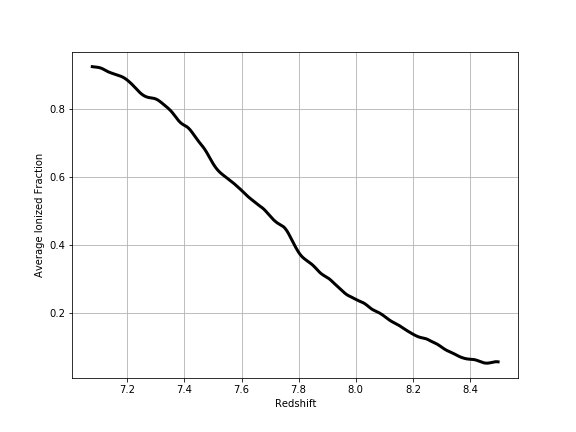
\includegraphics[width=0.6\textwidth]{chapters/ksz_21cm/figures/smoothed_ionfrac.png}
\caption{The average ionized fraction as a function of redshift in our cosmological simulation.}
\label{fig:ksz_21cm_sim_ionfrac_avg}
\end{figure}

\begin{figure}
\centering
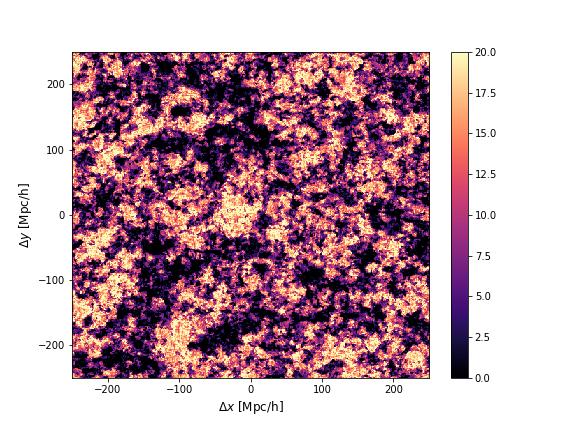
\includegraphics[width=0.49\textwidth]{chapters/ksz_21cm/figures/21cmExample_z7p8.png}
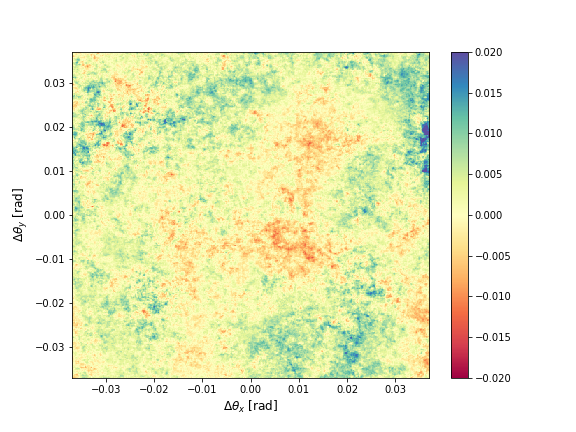
\includegraphics[width=0.49\textwidth]{chapters/ksz_21cm/figures/kszmap.png}
\caption[An example 21\,cm brightness temperature field and integrated kSZ map from our cosmological simulation.]{An example 21\,cm brightness temperature field at redshift $z\sim$7.8 (left) and integrated kSZ map (right) from our cosmological simulation. Both have color bars in units of mK.}
\label{fig:ksz_21cm_sim_example}
\end{figure}

\section{kSZ$^2$-21cm squeezed-triangle bispectra}
\label{sec:bispec}

In this section we present an estimate for bispectra formed from future HERA 21\,cm intensity maps (large scales; $\ell < 300$) and Stage 3 or 4 CMB maps (smaller scales; $\ell > 3000$). These disparate scales stretch the three-point correlation function into a `squeezed triangle' in Fourier space.

\subsection{Semi-analytic approximation}
\label{subsec:ksz_21cm_semi_analytic_approximation}

Consider the bispectrum of two Fourier transformed kSZ maps and one Fourier transformed 21\,cm map under the Limber approximation:
\begin{equation}
\begin{split}
 \left\langle T_{\rm kSZ}(\ell_1) T_{kSZ}(\ell_2) T_{\rm 21cm}(\ell_3)\right\rangle &= 
(2\pi)^2 \delta_D(\ell_1 + \ell_2 + \ell_3) \times \int
 \frac{{\rm d}\chi}{\chi^4} W_{\rm 21cm}(\chi) W_{\rm kSZ}^2(\chi)  \\
 & \times B_{\rm 21cm, kSZ, kSZ}(\ell_1/\chi, \ell_2/\chi,  \ell_3/\chi; \chi)
\label{eq:bispec_limber}
\end{split}
\end{equation}
where the window functions are based on global quantities associated with the maps:

\begin{equation}
W_{\rm 21cm}(\chi) = {\rm \frac{d}{d\chi}}\left(T_{\rm 21cm}(z)\right)
\label{eq:W21cm}
\end{equation}
where ${\rm d\chi}$ is the comoving distance probed by the 21\,cm map, given by the observing bandwidth, and

\begin{equation}
W_{\rm kSZ}(\chi) = T_{\rm CMB} \frac{\sigma_T n_e(z)}{c}\frac{\left\langle x_i \right\rangle e^{-\left\langle \tau(z) \right\rangle } }{1+z}
\label{eq:WkSZ}
\end{equation}
where redshift \textit{z} corresponds to a given comoving distance $\chi$, as determined by the central redshift of the 21\,cm cube, $n_e(z)$ is the average number density of electrons at that redshift, $\left\langle x_i \right\rangle $ is the average ionization fraction at that redshift, $\sigma_T$ is the Thomson cross section and $\tau (z)$ is the optical depth to redshift \textit{z}. $T_{\rm CMB} = 2.725\pm0.002$\,K \citep{Mather.99}.

Now we consider the Limber approximation of a related quantity: the 21\,cm field correlated with the square of the line-of-sight-projected momentum field:

\begin{equation}
\begin{split}
\left\langle \vec{q} \cdot \hat{n}(\vec{k}_1) \vec{q} \cdot \hat{n} (\vec{k}_2) T_{\rm 21cm}(\vec{k}_3) \right\rangle =
\int \int \frac{ {\rm d^3k' \, d^3k''} }{(2\pi)^6} (\hat{k'}\cdot\hat{n}) (\hat{k''}\cdot\hat{n}) \times \\
\left\langle 
\vec{v}(\vec{k'})\vec{v}(\vec{k''}) 
\left[ \delta_x(\vec{k}_1 - \vec{k'}) + \delta_{\rho}(\vec{k}_1 - \vec{k'})\right]
\left[ \delta_x(\vec{k}_2 - \vec{k''}) + \delta_{\rho}(\vec{k}_2 - \vec{k''})\right] 
T_{\rm 21cm}(\vec{k}_3)
\right\rangle
\end{split}
\label{eq:q_n_21}
\end{equation}
where we shifted our concentration from $\ell$ space to $\vec{k}$-space, which was more convenient to work in for the derivations below.
One of our assumptions in Section~\ref{sec:ksz-21cm} was that the velocity was coherent on large scales, and therefore should not correlate with $\delta_{x}$ or $\delta_{\rho}$. This allows us to expand the $[...]$ terms in Equation~\ref{eq:q_n_21} in their own spatial averages, and take the product of velocities into its own spatial average:

\begin{equation}
\left\langle \vec{v}(\vec{k'})\vec{v}(\vec{k''}) \right\rangle = (2\pi)^3 \delta_D(\vec{k'} + \vec{k''})P_{vv}(\vec{k'})
\label{eq:Pvv}
\end{equation}
where the $\delta_D(\vec{k'} + \vec{k''})$ in the above relation allowed us to integrate-out our $k''$ dependence. Referring to terms of the form $\langle \delta_i(\vec{k}_1 - \vec{k'}) \delta_j(\vec{k}_2 - \vec{k''}) \delta_{\rm 21cm}\rangle$ as $B_{i,j,{\rm 21cm}}$, we could express the overall correlator $\left\langle \vec{q} \cdot \hat{n}(\vec{k}_1) \vec{q} \cdot \hat{n} (\vec{k}_2) T_{\rm 21cm}(\vec{k}_3) \right\rangle$ in terms of ``component bispectra":

\begin{equation}
\begin{split}
\left\langle \vec{q} \cdot \hat{n}(\vec{k}_1) \vec{q} \cdot \hat{n} (\vec{k}_2) T_{\rm 21cm}(\vec{k}_3) \right\rangle &= 
(2\pi)^3 \delta_D(\vec{k}_1 + \vec{k}_2 + \vec{k}_3) \times \\
& \int \frac{{\rm d^3}k'}{(2\pi)^3} (\hat{k'}\cdot\hat{n})^2 P_{vv}(k') 
\left[ B_{x,x,\rm 21cm} + B_{x,\rho,\rm 21cm} + B_{\rho,x,\rm 21cm} +B_{\rho,\rho,\rm 21cm} \right].
\end{split}
\end{equation}

In the squeezed-triangle limit, where $k_3 << k_1,k_2$, this reduced to:
\begin{equation}
\begin{split}
\left\langle \vec{q} \cdot \hat{n}(\vec{k}_1) \vec{q} \cdot \hat{n} (\vec{k}_2) T_{{\rm 21cm}}(\vec{k}_3) \right\rangle &= 
(2\pi)^3 \delta_D(\vec{k}_1 + \vec{k}_2 + \vec{k}_3) \times \\
& \frac{v_{\rm rms}^2}{3} 
\left[ B_{x,x,{\rm 21cm}} + B_{x,\rho,{\rm 21cm}} + B_{\rho,x,{\rm 21cm}} +B_{\rho,\rho,{\rm 21cm}} \right]
\end{split}
\label{eq:component_bispectra}
\end{equation}

Of course, $\delta_{\rm 21cm}$ also contains information about $\delta_x$ and $\delta_{\rho}$. Using Equation~\ref{eq:d21cm_x}, we expanded each component bispectrum as functions of $\delta_x$, $\delta_{\rho}$ and $\delta_x\delta_{\rho}$:

\begin{equation}
\begin{split}
B_{x,x,{\rm 21cm}} &\propto B_{x,x,x} + B_{x,x,\rho} + B_{x,x,x\rho}\\
B_{x,\rho,{\rm 21cm}} &\propto B_{x,\rho,x} + B_{x,\rho,\rho} + B_{x,\rho,x\rho}\\
B_{\rho,x,{\rm 21cm}} &\propto B_{\rho,x,x} + B_{\rho,x,\rho} + B_{\rho,x,x\rho}\\
B_{\rho,\rho,{\rm 21cm}} &\propto B_{\rho,\rho,x} + B_{\rho,\rho,\rho} + B_{\rho,\rho,x\rho}\\
\end{split}
\label{eq:lots_of_bispectra}
\end{equation}
where the third index corresponds to large scales, and the first and second indices are probing the same small scale. To gain intuition for what to expect from simulations, we could make some approximations that allow us to reduce each subcomponent bispectrum into power spectra, which are inexpensively estimated from simulations.

\subsubsection{$B_{x,x,\rm 21cm}$}
\label{subsec:B_xx21}
Using Equations~\ref{eq:d21cm_x} and \ref{eq:bispec_limber}, we could write:
\begin{multline}
\langle \delta_x(\vec{k}_1) \delta_x(\vec{k}_2) \delta_{{\rm 21cm}}(\vec{k}_3) \rangle = 
\langle
T_0(1- \left\langle x_i \right\rangle ) \times \\
\left[
- \frac{\left\langle x_i \right\rangle}{1 - \left\langle x_i \right\rangle} \delta_x(\vec{k}_1) \delta_x(\vec{k}_2) \delta_x(\vec{k}_3) + \delta_x(\vec{k}_1) \delta_x(\vec{k}_2) \delta_{\rho}(\vec{k}_3) 
 - \frac{\left\langle x_i \right\rangle}{1 - \left\langle x_i \right\rangle} \delta_x(\vec{k}_1) \delta_x(\vec{k}_2) \int \frac{{\rm d^3}k'}{(2\pi)^3} \delta_x(\vec{k}_3 - \vec{k'})\delta_{\rho}(\vec{k'})
\right] \\
\times \delta_D(\vec{k}_1+\vec{k}_2+\vec{k}_3) 
\rangle .
\label{eq:B_xx21}
\end{multline}

Taking the averages inside the square brackets reduces all the terms to the to component bispectra written in Equation~\ref{eq:lots_of_bispectra}. The first and second terms are simpler to understand, whereas the third term contains a convolution left-over from Fourier transforming $\delta_x(\vec{x})\delta_{\rho}(\vec{x})$ from Equation~\ref{eq:d21cm_x}:

\begin{equation}
\begin{split}
B_{x,x,{\rm 21cm}} = \left( -T_0 \left\langle x_i \right\rangle B_{x,x,x} + T_0(1-\left\langle x_i \right\rangle) B_{x,x,\rho} - T_0 \left\langle x_i \right\rangle \int \frac{{\rm d^3}k'}{(2\pi)^3}
\langle \delta_x(\vec{k}_1) \delta_x(\vec{k}_2) \delta_x(\vec{k}_3 - \vec{k'})\delta_{\rho}(\vec{k'}) \rangle \right)\\
\times \delta_D(\vec{k}_1+\vec{k}_2+\vec{k}_3)
\end{split}
\end{equation}

\subsubsection*{$B_{x,x,x}$}
\label{subsubsec:Bxxx}
Consider the bispectrum $\langle\delta_x(\vec{k}_1)\delta_x(\vec{k}_2)\delta_x(\vec{k}_3)\rangle$. In the squeezed triangle limit of $k_3 << k_1, k_2$, we concentrated on the correlator

\begin{equation}
\langle \langle \delta_x(\vec{k}_1)\delta_x(\vec{k}_2) | \delta_x(\vec{k}_3)\rangle \delta_x(\vec{k}_3) \rangle
\end{equation}
This could be interpreted as: what is the correlation between expectation value of $\delta_x(\vec{k}_1)\delta_x(\vec{k}_2)$ given that $\delta_x(\vec{k}_3)$ has some value, with the ionization overdensity field $\delta_x(\vec{k}_1)$? If $\delta_x(\vec{k}_3)$ is sufficiently small, the expectation value may be expanded as a Taylor Series:

\begin{equation}
\langle \delta_x(\vec{k}_1)\delta_x(\vec{k}_2) | \delta_x(\vec{k}_3)\rangle =
\langle \delta_x(\vec{k}_1)\delta_x(\vec{k}_2) \rangle + 
\delta_x(\vec{k}_3) \frac{{\rm d}\langle\delta_x(\vec{k}_1)\delta_x(\vec{k}_2) | \delta_x(\vec{k}_3)\rangle}{{\rm d}\delta_x(\vec{k}_3)}|_{\delta_x(\vec{k}_3)=0} + \ldots.
\end{equation}

We could evaluate the derivative by assuming that the small-scale power $P_{\delta_x,\delta_x}(\vec{k_1}) = \langle \delta_x(\vec{k}_1)\delta_x(\vec{k}_2) \rangle$ in a large-scale ionized region is \textit{identical} to a typical region some time later when $\left\langle x_i \right\rangle$ has increased. This allows us to express the subcomponent bispectrum as 

\begin{equation}
B_{x,x,x} \approx P_{\delta_x,\delta_x}(\vec{k_3}) \frac{\partial P_{\delta_x,\delta_x}(\vec{k_2}) }{\partial\delta_x}|_{x_i = \left\langle x_i \right\rangle}
\end{equation}

Using the definition of $\delta_x = (x_i - \left\langle x_i \right\rangle)/\left\langle x_i \right\rangle$, we can rewrite the derivative with respect to $\left\langle x_i \right\rangle$ and use the chain rule
\begin{equation}
B_{x,x,x} = P_{\delta_x,\delta_x}(\vec{k_1}) P_{\delta_x,\delta_x}(\vec{k_3}) \left\langle x_i \right\rangle \frac{{\rm d} \ln (P_{\delta_x,\delta_x}(\vec{k_1}))}{{\rm d}\left\langle x_i \right\rangle}
\end{equation}

\subsubsection*{$B_{x,x,\rho}$}
\label{subsubsec:Bxxrho}
This subcomponent could be neglected for our estimate, since large-scale $\delta_{\rho}$ should be negligible.

\subsubsection*{$B_{x,x,x\rho}$}
\label{subsubsec:B_xxxrho}
The third term of $B_{x,x,{\rm 21cm}}$ takes the unflattering form of

\begin{equation}
- T_0 \left\langle x_i \right\rangle \int \frac{{\rm d^3}k'}{(2\pi)^3} 
\langle \delta_x(\vec{k}_1) \delta_x(\vec{k}_2) \delta_x(\vec{k}_3 - \vec{k'})\delta_{\rho}(\vec{k'}) \rangle .
\end{equation}

Making the assumption that all our fields are Gaussian\footnote{This is a highly-idealistic assumption, but allows the mathematics to be tangible. For a fast estimator this is acceptable, but it should not be interpreted as extremely physically motivated.}, we could expand the four-point function as three products of two-point functions. Evaluating them one-at-a-time:

\begin{equation}
\int \frac{{\rm d^3}k'}{(2\pi)^3} \langle \delta_x(\vec{k}_1) \delta_x(\vec{k}_2) \rangle \langle \delta_x(\vec{k}_3 - \vec{k'})\delta_{\rho}(\vec{k'}) \rangle
\end{equation}
This vanishes, since the integration of the second term picks-out the $\vec{k}_3 = \vec{k'}$ mode. Under the squeezed triangle approximation we can send $k_3 \rightarrow 0$, and $\delta_{\rho}(k'=0)=0$.

\begin{equation}
\int \frac{{\rm d^3}k'}{(2\pi)^3} \langle \delta_x(\vec{k}_1)\delta_x(\vec{k}_3 - \vec{k'}) \rangle \langle \delta_x(\vec{k}_2) \delta_{\rho}(\vec{k'}) \rangle \approx P_{\delta_x, \delta_x}(\vec{k}_1) P_{\delta_x, \delta_{\rho}}(\vec{k}_2) 
\end{equation}
The integration of the first term selects the $\vec{k_1} + \vec{k_3} = \vec{k'}$ mode. Under the squeezed triangle approximation, $\vec{k_1} \approx \vec{k'}$.

The third integral was just a permutation of the second, above. This meant that we can write the third subcomponent bispectrum as

\begin{equation}
-T_0 \left\langle x_i \right\rangle \left(P_{\delta_x, \delta_x}(\vec{k}_1) P_{\delta_x, \delta_{\rho}}(\vec{k}_2)  + P_{\delta_x, \delta_{\rho}}(\vec{k}_1) P_{\delta_x, \delta_x}(\vec{k}_2)  \right)
\end{equation}
and the component bispectrum from this subsection can be expressed as
% OVERFLOW
\begin{multline}
B_{x,x,{\rm 21cm}} \approx 
 - T_0 \left\langle x_i \right\rangle P_{\delta_x,\delta_x}(\vec{k_1}) \times \\
\left(
P_{\delta_x,\delta_x}(\vec{k_3}) \left\langle x_i \right\rangle \frac{{\rm d} \ln (P_{\delta_x,\delta_x}(\vec{k_1}))}{{\rm d}\left\langle x_i \right\rangle} 
+ P_{\delta_x, \delta_{\rho}}(\vec{k}_2)  +\frac{ P_{\delta_x, \delta_{\rho}}(\vec{k}_1)P_{\delta_x, \delta_x}(\vec{k}_2)}{P_{\delta_x,\delta_x}(\vec{k_1}) } 
\right) \\
\times \delta_D(\vec{k}_1+\vec{k}_2+\vec{k}_3)
\end{multline}

\subsubsection{$B_{x,\rho,{\rm 21cm}}$ and $B_{x,\rho,{\rm 21cm}}$}
\label{subsec:B_xrho21}

In the squeezed triangle limit, these two component bispectra are identical. Their joint contribution can be expressed as:
% OVERFLOW !!!
\begin{multline}
2\langle \delta_x(\vec{k}_1) \delta_x(\vec{k}_2) \delta_{{\rm 21cm}}\rangle = 
2T_0(1-\left\langle x_i \right\rangle) \\ \left\langle 
- \frac{\left\langle x_i \right\rangle}{1-\left\langle x_i \right\rangle} \delta_x(\vec{k}_1) \delta_{\rho}(\vec{k}_2) \delta_x(\vec{k}_3)
+ \delta_x(\vec{k}_1) \delta_{\rho}(\vec{k}_2) \delta_{\rho}(\vec{k}_3)
- \frac{\left\langle x_i \right\rangle}{1-\left\langle x_i \right\rangle} \delta_x(\vec{k}_1) \delta_{\rho}(\vec{k}_2) \int \frac{{\rm d^3}k'}{(2\pi)^3} \delta_x(\vec{k}_3 - \vec{k'})\delta_{\rho}(\vec{k'})\right\rangle
\end{multline}

\subsubsection*{$B_{x,\rho,x}$}
\label{subsubsec:Bxrhox}
We could follow a similar line of reasoning as in Section~\ref{subsubsec:Bxxx} by assuming that the small-scale $\delta_x\delta_{\rho}$ cross-power in an ionized region is the same as a typical region some time later when $\langle x_i \rangle$ has increased. This allowed us to express:

\begin{equation}
B_{x,\rho,x} \approx P_{\delta_x,\delta_{\rho}}(\vec{k}_1) P_{\delta_x,\delta_x}(\vec{k}_3)\left\langle x_i \right\rangle \frac{{\rm d} \ln (P_{\delta_x,\delta_{\rho}}(\vec{k_1}))}{{\rm d}\left\langle x_i \right\rangle}
\end{equation}

\subsubsection*{$B_{x,\rho,\rho}$}
\label{subsubsec:Bxrhorho}
This subcomponent could be neglected for our estimate, since large-scale $\delta_{\rho}$ should be negligible.

\subsubsection*{$B_{x,\rho,x\rho}$}
\label{subsubsec:Bxrhoxrho}

Following the same reasoning as in Section~\ref{subsubsec:B_xxxrho}, we arrived at the expression

\begin{equation}
\delta_x(\vec{k}_1)\delta_{\rho}(\vec{k}_2) \int \frac{\rm{d}k'}{(2\pi)^3}\delta_x(\vec{k}_3-\vec{k'})\delta_{\rho}(\vec{k'})
\approx
P_{\delta_x,\delta_x}(\vec{k}_1)P_{\delta_{\rho},\delta_{\rho}}(\vec{k}_2) + P_{\delta_x,\delta_{\rho}}(\vec{k}_1)P_{\delta_x,\delta_{\rho}}(\vec{k}_2)
\end{equation}
so the component bispectrum from this subsection can be expressed as

\begin{equation}
\begin{split}
-2 T_0 \left\langle x_i \right\rangle \left( P_{\delta_x,\delta_{\rho}}(\vec{k}_1) P_{\delta_x,\delta_x}(\vec{k}_3)\left\langle x_i \right\rangle \frac{{\rm d} \ln (P_{\delta_x,\delta_{\rho}}(\vec{k_1}))}{{\rm d}\left\langle x_i \right\rangle} +  P_{\delta_x,\delta_x}(\vec{k}_1)P_{\delta_{\rho},\delta_{\rho}}(\vec{k}_2) + P_{\delta_x,\delta_{\rho}}(\vec{k}_1)P_{\delta_x,\delta_{\rho}}(\vec{k}_2) \right) \\ 
\times \delta_D(\vec{k}_1+\vec{k}_2+\vec{k}_3)
\end{split}
\end{equation}

\subsubsection{$B_{\rho,\rho,{\rm 21cm}}$}
\label{subsec:B_rhorho21}

This component bispectrum was much simpler to calculate, as we expected the overdensity power to be subdominant to the ionization field.

\subsubsection*{$B_{\rho,\rho,x}$}
\label{subsubsec:Brhorhox}
Following results from Section~\ref{subsubsec:B_xxxrho}, this should be negligible so long as $P_{\delta_{\rho},\delta_{\rho}}(\vec{k}_1) < P_{\delta_{x},\delta_{x}}(\vec{k}_1)$, as expected.

\subsubsection*{$B_{\rho,\rho,\rho}$}
\label{subsubsec:Brhorhorho}
This subcomponent could be neglected for our estimate, since large-scale $\delta_{\rho}$ should be negligible.

\subsubsection*{$B_{\rho,\rho,x\rho}$}
\label{subsubsec:Brhorhoxrho}

As in Sections~\ref{subsubsec:B_xxxrho} and \ref{subsubsec:Bxrhoxrho}, we could take advantage of the convolution term in the Fourier transform to obtain

\begin{equation}
\delta_x(\vec{k}_1)\delta_{\rho}(\vec{k}_2) \int \frac{\rm{d}k'}{(2\pi)^3}\delta_x(\vec{k}_3-\vec{k'})\delta_{\rho}(\vec{k'})
\approx
P_{\delta_{\rho},\delta_x}(\vec{k}_1)P_{\delta_{\rho},\delta_{\rho}}(\vec{k}_2) + P_{\delta_{\rho},\delta_{\rho}}(\vec{k}_1)P_{\delta_{\rho},\delta_x}(\vec{k}_2)
\end{equation}

So the overall component bispectrum is the above, multiplied by a factor of $-T_0\left\langle x_i \right\rangle$.

\subsubsection{Full estimator}

Under the above assumptions, and simplifying with the squeezed triangle $P_{f,f}(\vec{k}_1)\approx P_{f,f}(\vec{k}_2)$ for $f=[x,\rho]$, we obtained our estimate for the bispectrum:

\begin{multline}
B_{\rm kSZ, kSZ, {\rm 21cm}}(\vec{k}_1,\vec{k}_2,\vec{k}_3) \approx 
-2T_0\left\langle x_i \right\rangle \times \\
\left[
P_{\delta_x,\delta_x}(\vec{k}_1) \left( P_{\delta_x,\delta_x}(\vec{k}_3)\frac{\left\langle x_i \right\rangle}{2} \frac{{\rm d} \ln (P_{\delta_x,\delta_x}(\vec{k_1}))}{{\rm d}\left\langle x_i \right\rangle} + P_{\delta_x,\delta_{\rho}}(\vec{k}_1) + P_{\delta_{\rho},\delta_{\rho}}(\vec{k}_1) \right) \right. \\
\left.
+ P_{\delta_x,\delta_{\rho}}(\vec{k}_1) \left( P_{\delta_x,\delta_x}(\vec{k}_3)\left\langle x_i \right\rangle \frac{{\rm d} \ln (P_{\delta_x,\delta_{\rho}}(\vec{k}_1))}{{\rm d}\left\langle x_i \right\rangle} + P_{\delta_x,\delta_{\rho}}(\vec{k}_1) + P_{\delta_{\rho},\delta_{\rho}}(\vec{k}_1) \right)
\right] \\
\times \delta_D(\vec{k}_1+\vec{k}_2+\vec{k}_3).
\label{eq:ksz_full_estimator}
\end{multline}

Equation~\ref{eq:ksz_full_estimator} shows our estimator consists of several small-scale power spectral components `riding' a large-scale ionization fluctuation. In the expected situation that power spectra consisting of density fluctuation components are subdominant to ionization fluctuations, we may expect a maximum or minimum at the mid-point of reionization, where the gradient of ionization power with respect average ionization is at an extreme.

\subsection{Counting triangles}

The signal-to-noise of a bispectrum scales with $\sqrt{N_{\rm Tri}}$, where $N_{\rm Tri}$ is the number of triangles.
A closed triangle in $\ell$-space can be represented by a two-dimensional Dirac delta-distribution $\delta^{(2)}_{D}(\vec{\ell_1}+\vec{\ell_2}+\vec{\ell_3})$. A count of the different orientations of such a triangle was formulated by \cite{Joachimi.09} as:

\begin{equation}
\int^{2\pi}_0 {\rm d}\phi_{\ell1} \int^{2\pi}_0 {\rm d}\phi_{\ell2} \int^{2\pi}_0 {\rm d}\phi_{\ell3} \,\delta^{(2)}_{D}(\vec{\ell_1}+\vec{\ell_2}+\vec{\ell_3})
\end{equation}

Which can be represented as an exponential:

\begin{equation}
\begin{split}
\int^{2\pi}_0 {\rm d}\phi_{\ell1} \int^{2\pi}_0 {\rm d}\phi_{\ell2} \int^{2\pi}_0 {\rm d}\phi_{\ell3} \,\int^{\infty}_0 \frac{{\rm d^2\theta}}{(2\pi)^2}\exp\left(i(\vec{\ell_1}+\vec{\ell_2}+\vec{\ell_3})\cdot\vec{\theta}\right)\\
= (2\pi)^2\int^{\infty}_0 {\rm d}\theta \theta J_0(\ell_1\theta)J_0(\ell_2\theta)J_0(\ell_3\theta)
\end{split}
\end{equation}

Where they used the definition $J_0(x) = \int^{2\pi}_0 {\rm d}\phi e^{ix\cos\phi}/2\pi$. \cite{gradshteyn2000table} give the analytic solution for the final integral for closed-triangle configurations for triple products of any order of Bessel Function. For zeroth-order Bessel Functions, their solution reduces to the reciprocal of the area of the triangle:

\begin{equation}
(2\pi)^2\int^{\infty}_0 {\rm d}\theta \theta J_0(\ell_1\theta)J_0(\ell_2\theta)J_0(\ell_3\theta) = \left( \frac{1}{4}\sqrt{2\ell_1^2\ell_2^2 + 2\ell_1^2\ell_3^2 + 2\ell_2^2\ell_3^2 - \ell_1^4 - \ell_2^4 - \ell_3^4} \right)^{-1}
\end{equation}

In reality, measurements of any bispectrum or power spectrum will be binned in $\ell$, with central values and widths of $\bar{\ell}$ and $\Delta\ell$ respectively. The number of triangles in a kSZ$^2$-21cm bispectrum bin will be given by:

\begin{equation}
N_{\rm Tri} \approx 2\pi\Omega_S^2\bar{\ell_1}\bar{\ell_2}\bar{\ell_3}\Delta\ell_1\Delta\ell_2 \Delta\ell_3 \int^{\infty}_0 {\rm d}\theta \theta J_0(\bar{\ell_1}\theta)J_0(\bar{\ell_2}\theta)J_0(\bar{\ell_3}\theta)
\label{eq:Ntri}
\end{equation}

For the limits on $\ell_{1,2,3}$ mentioned at the beginning of Section~\ref{sec:bispec} concerning near-future CMB experiments and HERA's most-numerous short baselines, Equation~\ref{eq:Ntri} gives $N_{\rm Tri}\sim10^9$, for a sky fraction of 0.03, surveyed by the HERA drift-scanned stripe.

\subsection{Results}

The $P_{\delta_{\rho},\delta_{\rho}}(k)$, $P_{\delta_x,\delta_x}(k)$ and $P_{\delta_x,\delta_{\rho}}(k)$ power spectra relevant to the estimator are shown (from top to bottom) in Figure~\ref{fig:ksz_21cm_power_spectra_stuff} . The line colors, as labelled, correspond to different redshift slices from the simulation cube. As expected, the density power spectrum slowly increased in amplitude with decreasing redshift, as structure grew hierarchically.  The ionization power spectrum was highest at the midpoint of reionization, when there was maximal contrast in the brightness temperature field. This latter trend dominated their cross-power spectrum.

\begin{figure}
\centering
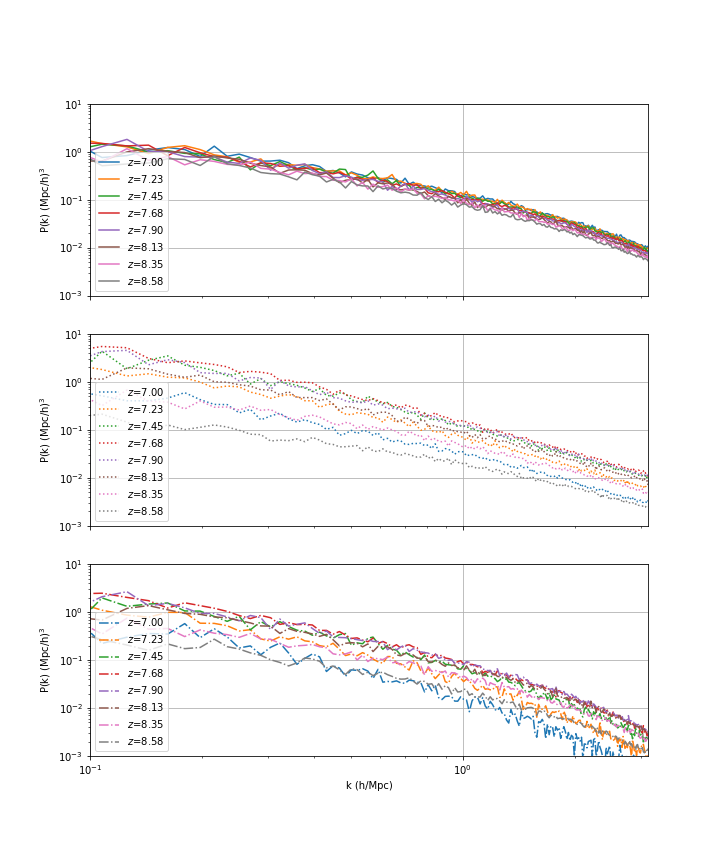
\includegraphics[width=0.8\textwidth]{chapters/ksz_21cm/figures/d_x_cross_powerspecs.png}
\caption[The $P_{\delta_{\rho},\delta_{\rho}}(k)$, $P_{\delta_x,\delta_x}(k)$ and $P_{\delta_x,\delta_{\rho}}(k)$ power spectra relevant to our semianalytic estimate of the bispectrum.]{The (top to bottom) $P_{\delta_{\rho},\delta_{\rho}}(k)$, $P_{\delta_x,\delta_x}(k)$ and $P_{\delta_x,\delta_{\rho}}(k)$ power spectra relevant to our semianalytic estimate of the bispectrum.}
\label{fig:ksz_21cm_power_spectra_stuff}
\end{figure}

Coupled with relevant derivatives with respect to ionization fraction, and averages with respect to redshift, we could use the power spectra above to calculate the estimator in Equation~\ref{eq:ksz_full_estimator} as a function of redshift -- shown in Figure~\ref{fig:ksz_21cm_semianalytic_result}. As expected, the magnitude of the estimated bispectrum is at an extreme close to the center of reionization. Also as expected, it is negative, showing that the 21\,cm and kSZ power are anti-correlated. It also appears to be quite noisy, with the large dip at $z\sim 7.3$ lacking a clear explanation.

\begin{figure}
\centering
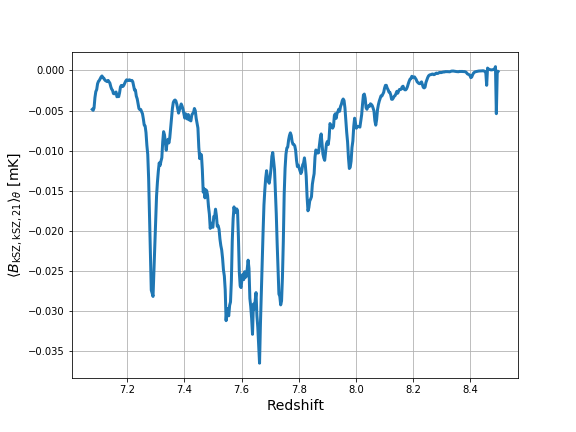
\includegraphics[width=0.65\textwidth]{chapters/ksz_21cm/figures/semianalytic_bispec_vs_z.png}
\caption{The semianalytic expression of the bispectrum, calculated as a function of redshift from our simulation.}
\label{fig:ksz_21cm_semianalytic_result}
\end{figure}

Of course, we were also able to calculate the bispectrum directly from the simulated 21\,cm and kSZ fields, restricting ourselves to relevant $\ell$ modes for HERA baselines and CMB experiments. However, we found that the box was too small to sample an appropriate number of large-scale modes, such that there were too few triangles in the box to converge on a given magnitude. In Figure~\ref{fig:ksz_21cm_direct_bispectrum}, we show bispectum power binned as a function of angle between the $\vec{k}$ vector for the 21\,cm field and one of the $\vec{k}$ vectors from the kSZ map (a dimension which our semianalytic estimator does not probe, as it uses power spectra and assumes the ultimate squeezed triangle limit of $\theta = 0$) from $z=7.6$. The values, while larger than the expected experimental noise\footnote{The signal to noise of the bispectrum is given by: \begin{equation}
\left(\frac{S}{N}\right)^2 = \frac{B(\ell_1, \ell_2, \ell_3)}{C_{\rm CMB}^N(\ell_1)C_{\rm CMB}^N(\ell_2)C_{\rm 21cm}^N(\ell_3)}
\end{equation}} by a factor of at least $10$, are consistent with numerical noise, oscillating about zero with high variance. This is true for all redshifts probed.

\begin{figure}
\centering
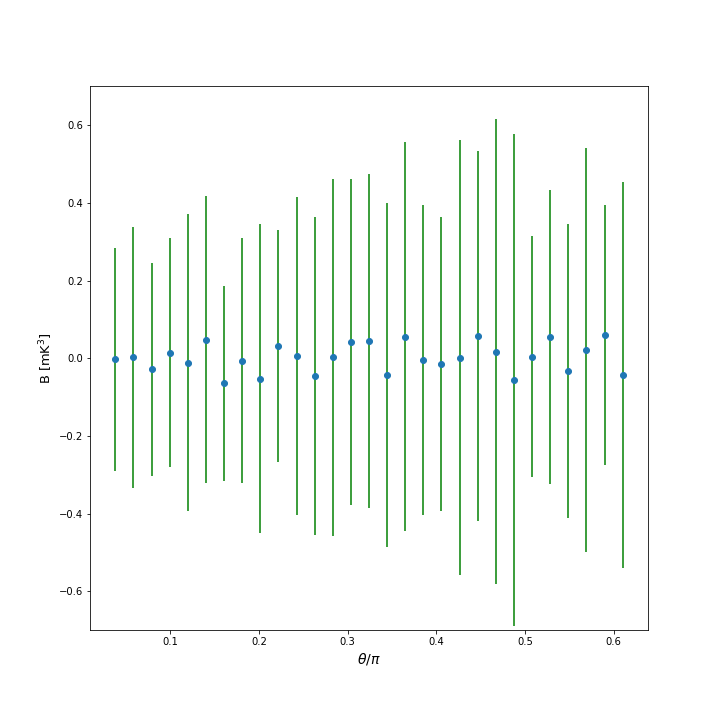
\includegraphics[width=0.65\textwidth]{chapters/ksz_21cm/figures/analytic_bispec_decimate1.png}
\caption[Bispectrum values, binned as a function of angle between the 21\,cm and CMB $\vec{k}$ vectors, measured directly from the simulation.]{Bispectrum values, binned as a function of angle between the 21\,cm and CMB $\vec{k}$ vectors, measured directly from the simulation at $z=7.6$. The values are consistent with zero, most likely due to too few large-scale modes present in the cube.}
\label{fig:ksz_21cm_direct_bispectrum}
\end{figure}

% w.r.t redshift???

Figure~\ref{fig:ksz_21cm_direct_bispectrum} highlights one of the limitations of using the bispectrum as a statistic to probe reionization. It is difficult to obtain sufficient numbers of triangles in a simulation cube to converge on a bispectrum value. While it was possible to calculate the bispectrum for a single redshift on a $512^3$ resolution element box in minutes, running the same calculation on a $2048^3$ element box would take roughly six hours. This means that characterization of the bispectrum -- understanding its sensitivity to astrophysical and cosmological parameters -- is difficult to obtain, as this would require large numbers of simulations with varied parameters, large enough to produce higher signal-to-noise bispectra than we are capable of in this work. \cite{Sefusatti.16} and \cite{Watkinson.17} have suggested FFT-based estimators to overcome the poor scaling associated with bispectrum calculations; pursuing these methods in future investigations may prove worthwhile.

Possibly the largest limitation of the bispectrum is one that has been brushed under the carpet in most of the discussion above. The kSZ only exists in the $k_{\parallel}=0$ plane, since by its integral definition it has not line-of-sight component. Because two kSZ terms are required, this forces any closed triangle (enforced by the Dirac delta functions throughout Section~\ref{subsec:ksz_21cm_semi_analytic_approximation}) to exist only at $k_{\parallel}=0$ values: the 21\,cm component is trapped within the center of the wedge! One could argue that the foreground contamination problem is not strictly the same for the bispectrum as it is for the 21\,cm power spectrum, as the `true' foreground for the bispectrum is the correlation of the CMB with low-frequency Galactic synchrotron, which is low \citep[e.g.][]{Ichiki.14}. However, while the effective $T^2_{\rm sys}$ in Equation~\ref{eq:ksz_21cm_HERA_noise_total} is close to receiver noise outside of the wedge, at $k_{\parallel}=0$ its value becomes very large, as it is dominated by $T_{\rm sky}$. 

To be non-zero outside of the wedge, two 21\,cm fields are required in the correlation function. This moved us to a minimum four point function, which we explored with the trispectrum below.

\section{kSZ$^2$-21cm$^2$ squeezed-rectangle trispectra}
\label{sec:trispec}

As noted above, to correlate with a kSZ map, we have to square the it to force it to be positive-definite. If we use a single 21\,cm map to correlate with two kSZ maps (i.e. a bispectrum), we must satisfy a Dirac delta function of the form $\delta_D(\vec{k}_1 + \vec{k}_2 + \vec{k}_3)$. Since the kSZ is a projected quantity, it contains no line-of-sight modes, so two of the k vectors have no line-of-sight component; the third k vector must also have no line-of-sight component. That means that the 21\,cm contribution is stuck in the center of the wedge.

The trispectrum of these fields, with two 21\,cm maps and two kSZ maps, does not share this problem. Its Dirac delta function has two \textit{k} vectors associated with the 21\,cm field, and these can cancel each other to satisfy a closed-quadrilateral condition. We limit ourselves to discussion of the squeezed trispectrum, where the k modes of the 21cm field are much larger than the k modes of the kSZ field. This is a realistic regime for the combination of HERA with Stage 3 or 4 CMB experiments. The geometry of these statistics are shown in Figure~\ref{fig:ksz_21cm_correlation_geometries}. 

\begin{figure}
\centering
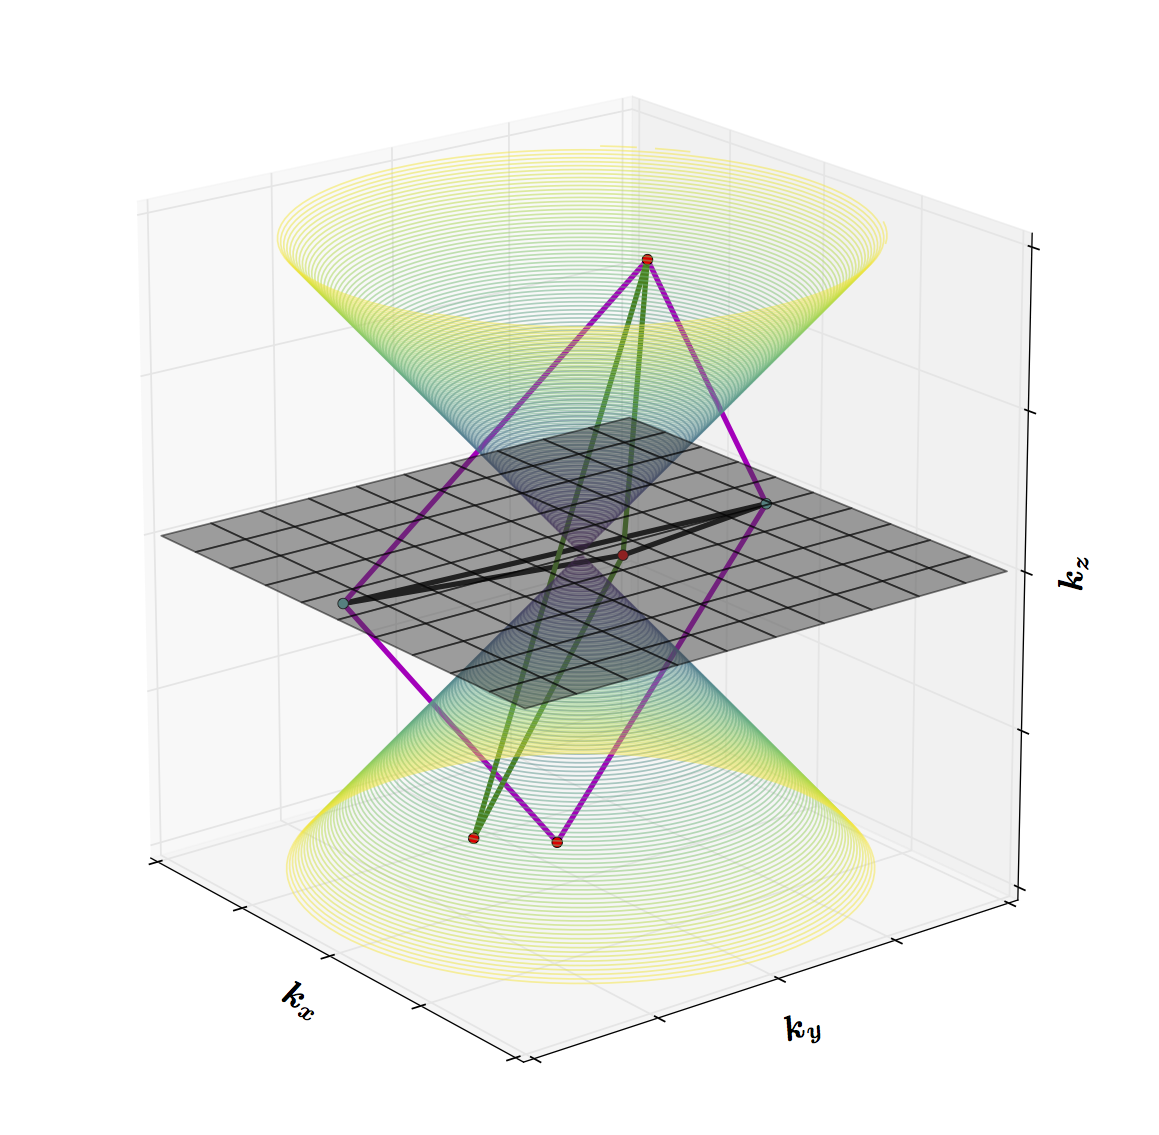
\includegraphics[width=0.5\textwidth]{chapters/ksz_21cm/figures/trispec_and_bispec_3d_fig.png}
\caption[The geometry of the correlation statistics considered in this Chapter.]{The geometry of the correlation statistics considered in this Chapter. The conical shape indicates the boundaries of the wedge in $k_x,k_y,k_z$ space (i.e. not cylindrically averaged into $k_{\perp},k_{\parallel}$), where being `within' the wedge is being outside of the boundaries. Closed triangles of the 21\,cm-kSZ$^2$ bispectrum are represented by the black lines -- because of the projected nature of the kSZ, they must exist within the wedge. 21\,cm$^3$ bispectra, the green lines, could potentially recover 21\,cm statistics from within the wedge. 21\,cm$^2$-kSZ$^2$ trispectra, the magenta lines, allow us to correlate the 21\,cm signal and the kSZ without the limitations of working within foreground-contaminated regions.}
\label{fig:ksz_21cm_correlation_geometries}
\end{figure}

\subsection{Mathematical formulation}

The trispectrum can be written as follows (note that in terms such as $\vec{k}^2_{\perp}$, the 2 is a label and not an exponent; we will define terms below):

\begin{equation}
\begin{split}
\mathcal{T}(\delta^{2D}_{\rm 21\,cm}, \delta^{2D}_{\rm 21\,cm}, \delta_{\rm kSZ}, \delta_{\rm kSZ}; z) &=
\langle \delta^{2D}_{\rm 21\,cm}(\vec{k}^1_{\perp})  \delta^{2D}_{\rm 21\,cm}(\vec{k}^2_{\perp})  \delta_{\rm kSZ}(\vec{k}^3_{\perp})\delta_{\rm kSZ}(\vec{k}^4_{\perp}) \rangle \\
&=
\int \frac{{\rm d}k^1_{\parallel}}{2\pi} \frac{{\rm d}k^2_{\parallel}}{2\pi} \frac{{\rm d}k^3_{\parallel}}{2\pi} \frac{{\rm d}k^4_{\parallel}}{2\pi}
W_{\rm 21\,cm}(k^1_{\parallel}) W_{\rm 21\,cm}(k^2_{\parallel}) W_{\rm kSZ}(k^3_{\parallel}) W_{\rm kSZ}(k^4_{\parallel}) \\
&
\times \langle \delta^{3D}_{\rm 21\,cm}(k^1_{\parallel}, \vec{k}^1_{\perp}) \delta^{3D}_{\rm 21\,cm}(k^2_{\parallel}, \vec{k}^2_{\perp}) \delta_{\rm SZ}(k^3_{\parallel}, \vec{k}^3_{\perp})  \delta_{\rm SZ}(k^4_{\parallel}, \vec{k}^4_{\perp}) \rangle \\
&
\times \delta_D(\vec{k}^1 + \vec{k}^2 + \vec{k}^3 + \vec{k}^4)
\end{split}
\label{eq:overall_trispec}
\end{equation}
The window functions above represent the key motivation for calculating the trispectrum.
\begin{equation}
W_{\rm 21cm}(k_{\parallel}) = 
\begin{cases} 
      1 & k_{\parallel, {\rm min}}\leq k_{\parallel} \leq k_{\parallel, {\rm max}} \\
      0 & {\rm otherwise}
\end{cases},
\label{eq:trispec_W21_kpl}
\end{equation}
where $k_{\parallel, {\rm min}}$ is set by the interferometer baseline $\vec{b}$ and is the boundary of the wedge, and $k_{\parallel, {\rm max}}$ could take a range of values, the smallest of which proportional to the Fourier conjugate of a single frequency channel-width. This window function filters-out the wedge. $W_{\rm kSZ}$ is given by Equation~\ref{eq:WkSZ}. We represent the wedge-filtered 21\,cm field as
\begin{equation}
\delta^{2D}_{\rm 21\,cm}(\vec{k}_{\perp}) = \int \frac{{\rm d}k_{\parallel}}{2\pi} W_{\rm 21\,cm}(k_{\parallel}) \delta^{3D}_{\rm 21\,cm}(k_{\parallel}, \vec{k}_{\perp}).
\end{equation}

Equation~\ref{eq:overall_trispec} could be simplified. The Dirac delta functions may be factored into line-of-sight and transverse components,
\begin{equation}
\delta_D(\vec{k}^1 + \vec{k}^2 + \vec{k}^3 + \vec{k}^4) = \delta_D(k^1_{\parallel} + k^2_{\parallel} + k^3_{\parallel} + k^4_{\parallel})\delta_D(\vec{k}^1_{\perp} + \vec{k}^2_{\perp} + \vec{k}^3_{\perp} + \vec{k}^4_{\perp}).
\end{equation}
In the squeezed limit, $k^3_{\parallel},k^4_{\parallel} \ll k^1_{\parallel},k^2_{\parallel}$. This allowed us to use the Limber approximation for the kSZ window function, as written in Equation~\ref{eq:WkSZ}. 

We may also approximate the central $k$ mode picked-out by the 21\,cm window function in Equation~\ref{eq:trispec_W21_kpl} as a single $k_{\parallel,\alpha}$. We write $\delta^{3D}_{\rm 21\,cm}(k^{\alpha}_{\parallel},\vec{k_{\perp}}) = \delta^{2D}_{\rm 21\,cm,\alpha}(\vec{k}_{\perp})$.

Together these simplifications allowed three of the four integrations to be performed:
\begin{equation}
\begin{split}
\mathcal{T}(\delta^{2D}_{\rm 21\,cm}, \delta^{2D}_{21\,cm}, \delta_{\rm kSZ}, \delta_{\rm kSZ}; z) &= 
\langle \delta^{2D}_{\rm 21\,cm,\alpha}(\vec{k}^1_{\perp})  \delta^{2D}_{\rm 21\,cm,\alpha}(\vec{k}^2_{\perp})  \delta_{\rm kSZ}(\vec{k}^3_{\perp})\delta_{\rm kSZ}(\vec{k}^4_{\perp}) \rangle \\ 
& \times \delta_D(\vec{k}^1_{\perp} + \vec{k}^2_{\perp} + \vec{k}^3_{\perp} + \vec{k}^4_{\perp}) | W_{\rm kSZ}(z) |^2\int \frac{{\rm d}k^1_{\parallel}}{2\pi} | W_{\rm 21\,cm,\alpha} (k^1_{\parallel}) |^2
\end{split}
\label{eq:squeezed_trispec}
\end{equation}
%filtering stages - note abs of filtered data (since we lose the zero point)

\subsection{Effects of filtering}

It is valuable to note that filtering the 21\,cm and kSZ maps has a dire effect on how simple it is to interpret these objects in image space. As an illustration, in Figure~\ref{fig:effect_of_filtering_panels} we show a representative slice of our 21\,cm brightness temperature cube before and after wedge filtering, and the kSZ map before and after low- and high-pass filtering. The effect on the kSZ is relatively easy to understand -- most of the large diffuse features ($\ell < 3000$)are eliminated by the high-pass cutoff, while the low-pass is not as stringent ($\ell > 13000$), leaving only small-scale modes within the image. However, removing the wedge does not constitute a simple high or low-pass filter. Instead, power is shifted around in image-space. This effect lead to \cite{Beardsley.15} showing that a given cell in a wedge-filtered image can only be used to obtain a model-dependent estimate of the ionization fraction.

\begin{figure}
\centering
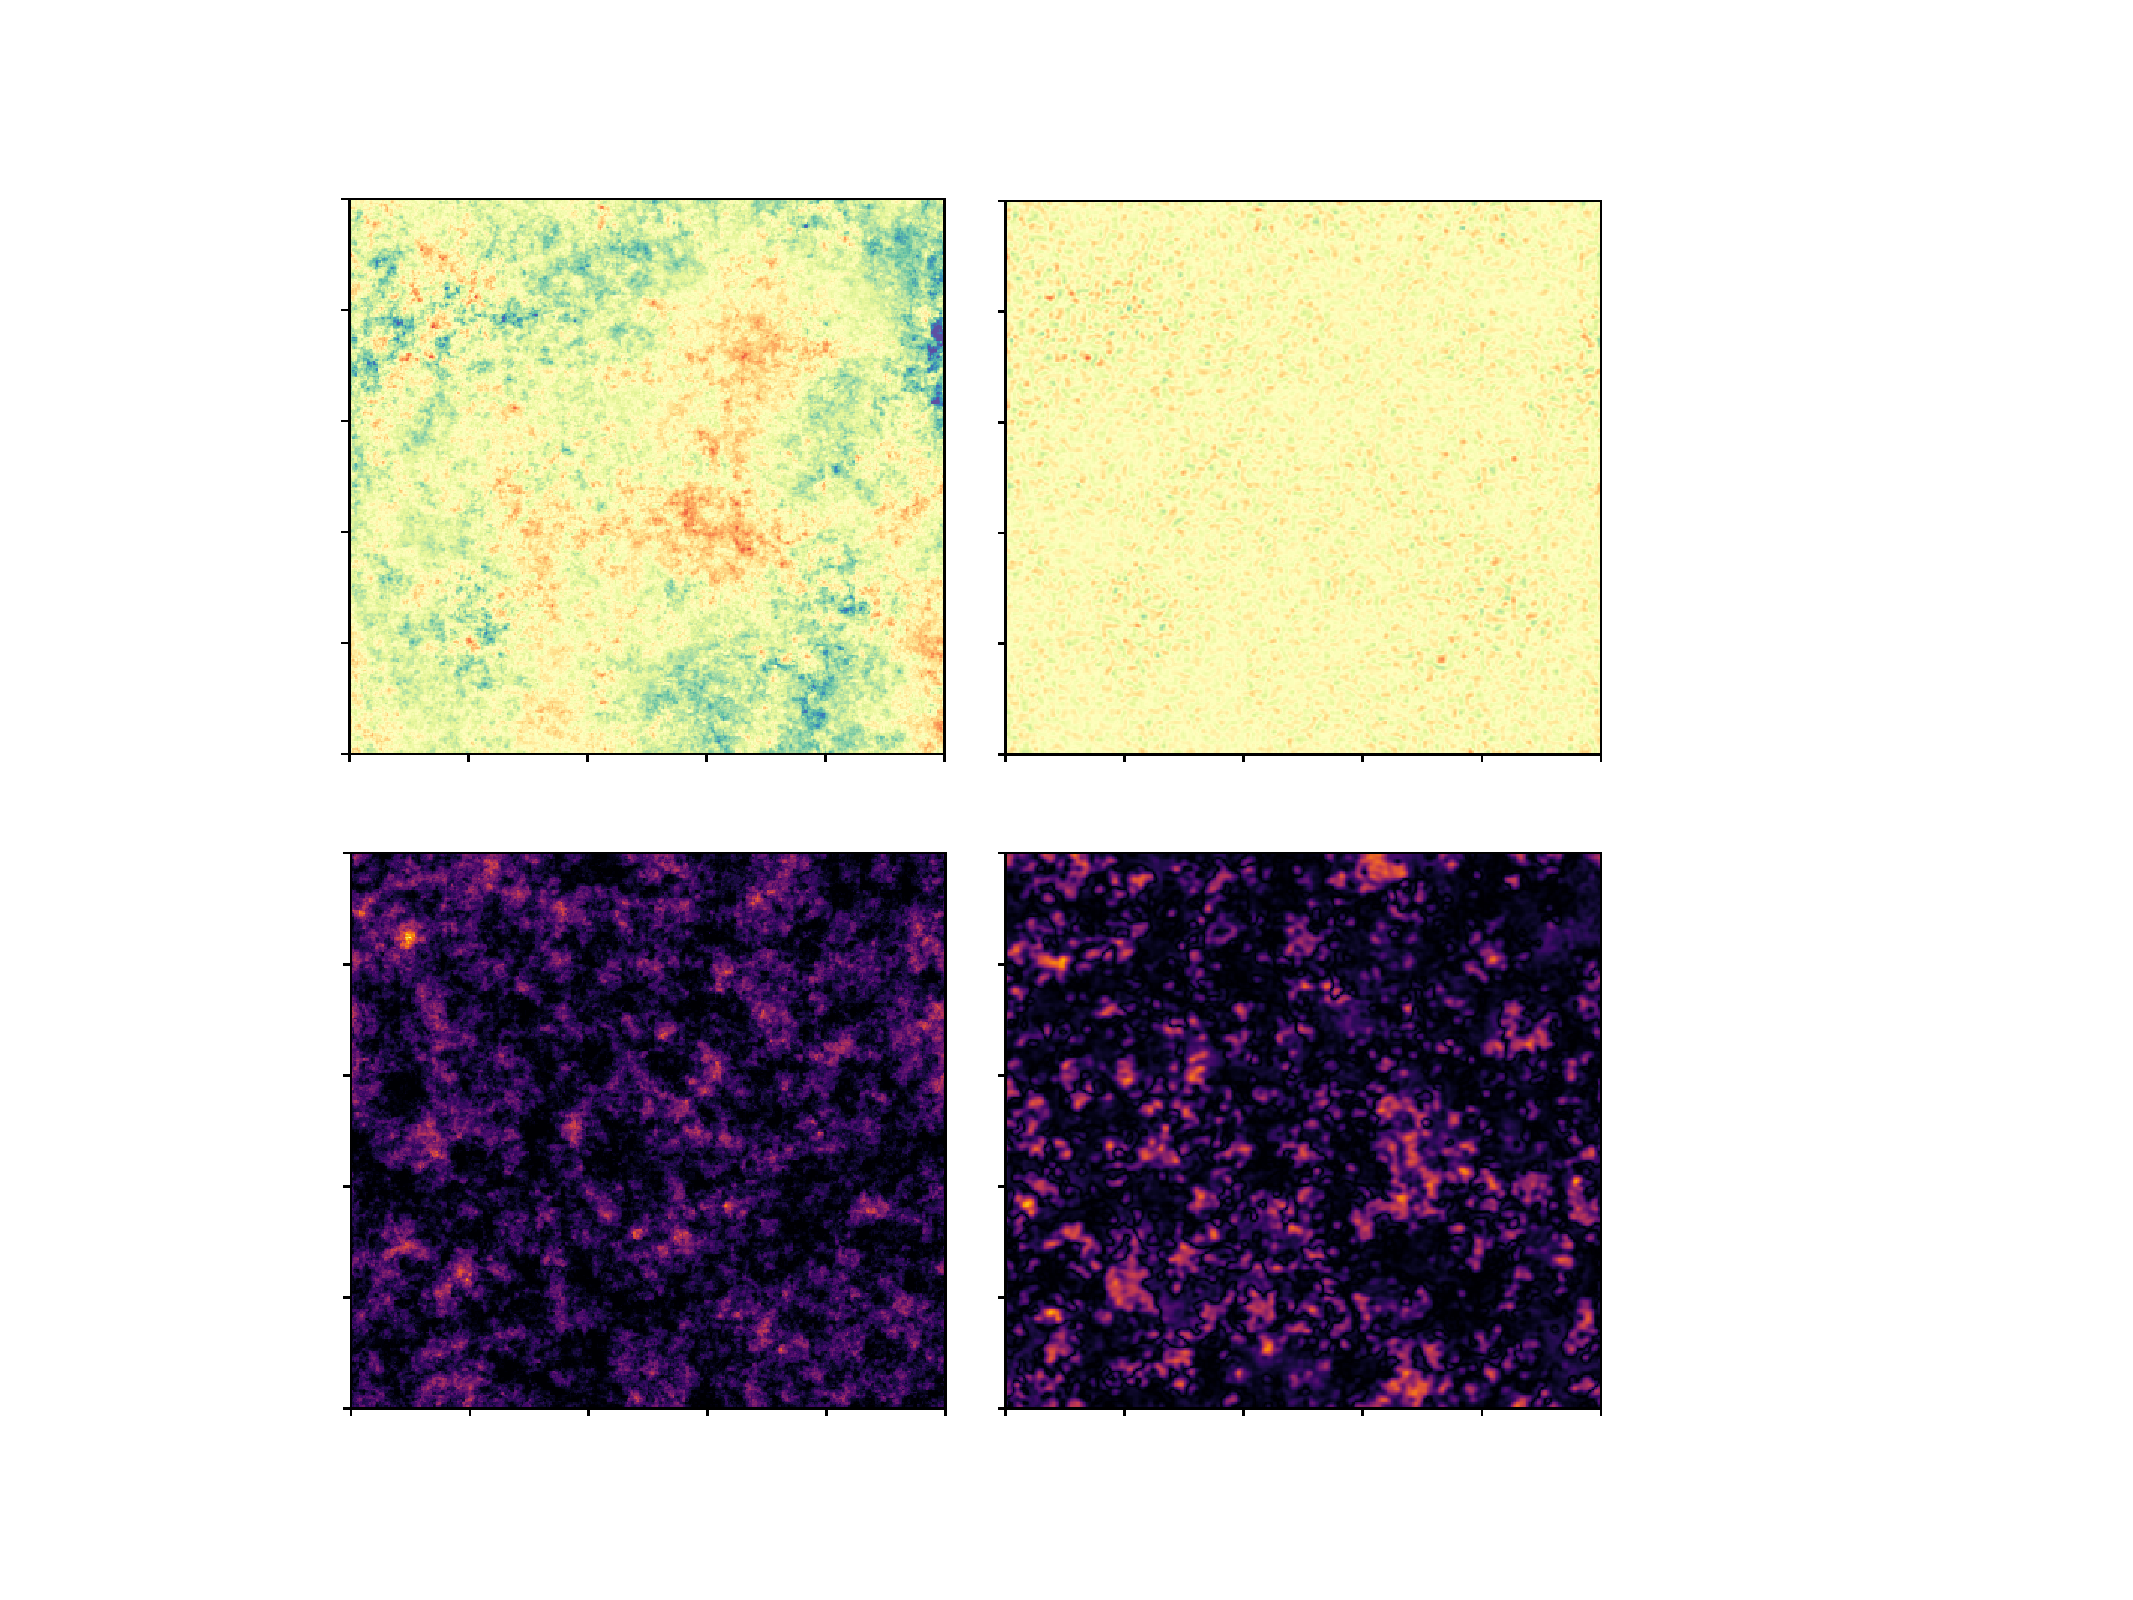
\includegraphics[width=0.8\textwidth]{chapters/ksz_21cm/figures/filter_compare.pdf}
\caption[The effect of filtering kSZ and 21cm maps to avoid foreground contamination.]{The effect of filtering kSZ and 21cm maps to avoid foreground contamination. Top panels are the kSZ map from our simulation, before (left) and after (right) high and low pass filtering. After filtering, only small-scale modes survive. The bottom panels show a slice of the 21\,cm brightness temperature cube before (left) and after (right) wedge-filtering. Power is entirely scrambled, and small-scale details are removed. The colorbars are matched for pre- and post- filtered maps.}
\label{fig:effect_of_filtering_panels}
\end{figure}

We can also see strange effects of wedge filtering more qualitatively by forming 1D power spectra of the 21\,cm$^2$ brightness temperature before and after the cube has been filtered. This is shown for several different redshifts in Figure~\ref{fig:effect_of_filtering_21squared}. As expected, removing modes from inside the wedge results in a decrease in power. However, the hierarchy of power as a function of redshift also changes after the filter. This lacks an easy explanation.

\begin{figure}
\centering
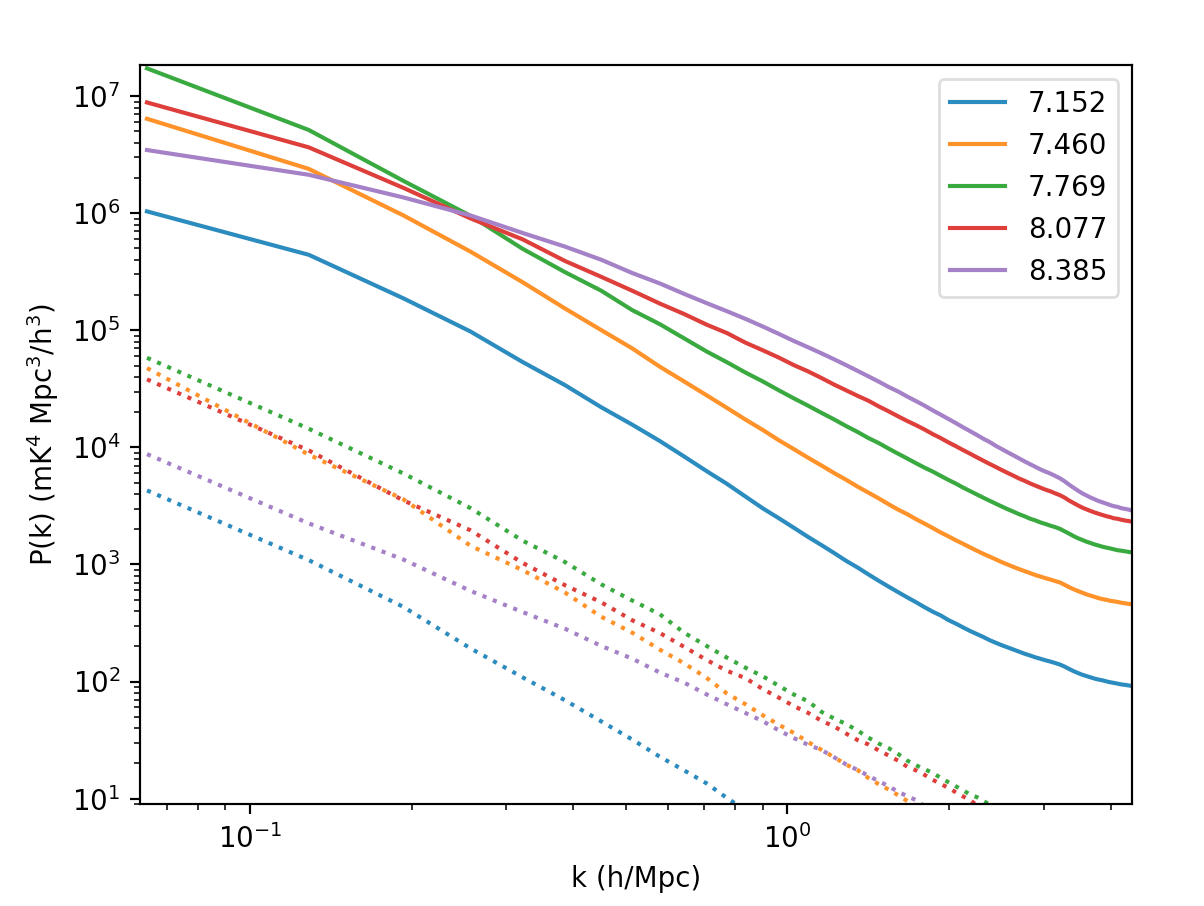
\includegraphics[width=0.6\textwidth]{chapters/ksz_21cm/figures/unfilt_filt_pspec21.png}
\caption[21\,cm$^2$ power spectra before and after filtering the wedge for several redshifts.]{21\,cm power spectra before (solid) and after (dotted) filtering the wedge for several redshifts. Not only does filtering the wedge decrease power, it also changes the hierarchy of power between power spectra, with respect to redshift.}
\label{fig:effect_of_filtering_21squared}
\end{figure} 

\subsection{kSZ$^2$-21cm$^2$ cross-power spectrum}

While bispectra are computationally costly to calculate, trispectra are even more so. However, unlike the bispectrum, the trispectrum lacks an easy-to-understand semianalytic estimator. When we applied the same tactics as used in Section~\ref{subsec:ksz_21cm_semi_analytic_approximation}, all terms vanished except for the `connected' Gaussian term, that we would need to subtract from our final trispectrum estimate in the end, anyway:
\begin{equation}
\Delta\mathcal{T} \approx P_{\rm 21cm}(vec{k}^1_{\perp})P_{\rm kSZ}(vec{k}^3_{\perp}) \times |W_{\rm kSZ}(z)|^2.
\end{equation}

However, the form of Equation~\ref{eq:squeezed_trispec} suggests that one term in the overall trispectrum that may be an interesting and efficient quantity to calculate is the cross-power spectrum between the squared 21\,cm and squared kSZ fields. Each would have to be filtered before squaring, in order to not convolve foreground-contaminated modes with otherwise clean ones. For the cross-spectrum of squared fields $P_X(k)$, we defined a ratio
\begin{equation}
r_k = \frac{P_X(k)}{\sqrt{P_{\rm 21cm^2}(k) + P_{\rm kSZ^2}(k)} }
\end{equation}
...
% what's the point of the ratio again?

% future work - 21\,cm bispectrum with one point inside the wedge